% Pontos A(0,0), B(2,0), C(6,0), D(8,0)
% Apoio fixo em A, apoio móvel em D
% 30kNm horário aplicado em A
% 10kN/m entre B e C

\documentclass[tikz]{standalone}
\usepackage{stanli}
\usetikzlibrary{calc}

\begin{document}
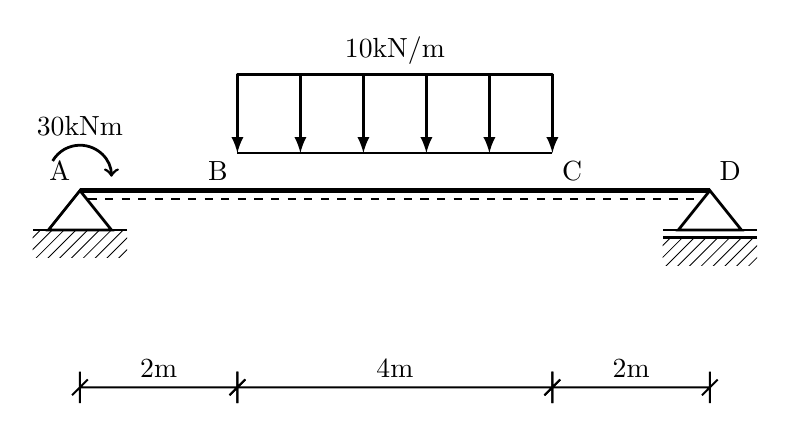
\begin{tikzpicture}
    % Definição dos pontos principais
    \point{A}{0}{0}
    \point{B}{2}{0}
    \point{C}{6}{0}
    \point{D}{8}{0}
    
    % Pontos auxiliares para evitar sobreposição de cargas e notações
    \point{A'}{0}{5pt}
    \point{B'}{2}{5pt}
    \point{C'}{6}{5pt}

    % Definição dos apoios
    \support{1}{A} % Apoio fixo em A
    \support{2}{D} % Apoio móvel em D

    % Definição da viga
    \beam{1}{A}{D}

    % Cargas
    % Momento horário de 30kNm em A
    \load{2}{A'}[0][150]
    
    % Carga distribuída de 10kN/m entre B e C
    \lineload{1}{B'}{C'}

    % Notações e Etiquetas
    \notation{1}{A}{A}[above left]
    \notation{1}{B}{B}[above left]
    \notation{1}{C}{C}[above right]
    \notation{1}{D}{D}[above right]
    
    % Rótulos de carga conforme instruções
    \notation{1}{A'}{30kNm}[above=4mm]
    \notation{5}{B'}{C'}[10kN/m][.5][above=13mm]

    % Dimensionamento (abaixo da estrutura para não colidir com as cargas)
    \dimensioning{1}{A}{B}{-25mm}[2m]
    \dimensioning{1}{B}{C}{-25mm}[4m]
    \dimensioning{1}{C}{D}{-25mm}[2m]
\end{tikzpicture}
\end{document}